\documentclass[10pt,a4paper]{article}
\usepackage[margin=17mm]{geometry}
\usepackage[T1]{fontenc}
\usepackage{lmodern}
\usepackage{microtype}
\usepackage{amsmath,amssymb}
\usepackage{booktabs}
\usepackage{graphicx}
\usepackage{caption}
\usepackage{xcolor}
\usepackage[hidelinks]{hyperref}
\usepackage{enumitem}

\graphicspath{{../figures/}{figures/}}
\captionsetup{font=small,labelfont=bf,skip=4pt}
\setlength{\parindent}{0pt}
\setlength{\parskip}{4pt}
\setlist[itemize]{leftmargin=*,nosep}
\newcommand{\se}{\mathop{\rm SE}}

\title{Final-pair statistics in higher-dimensional cyclic systems}
\author{Ruocun Ou\\\small Nanyang Normal University \quad \href{mailto:ouruocun@gmail.com}{ouruocun@gmail.com}}
\date{}

\begin{document}
\maketitle
\vspace{-1.6em}

\paragraph{Motivation.}
The three-species studies of cyclic competition with environmental switching by West, Mobilia and Rucklidge, and by West and Mobilia, prompted me to ask what can be seen if the full extinction sequence is recorded after extending the interaction cycle beyond three species.  The calculation below is a numerical exploration of that question.  It uses the birth--death formulation with a dichotomously switching carrying capacity from West and Mobilia (2020), but replaces the three-species payoff matrix by weighted antisymmetric nearest-neighbour cycles with odd $q=5,7,9$.  It is therefore not intended as a direct extension of every assumption or conclusion in either paper.

\paragraph{Process and measurements.}
Let $n_i$ be the abundance of species $i$, $M=\sum_i n_i$, and $x_i=n_i/M$.  Events are simulated exactly in continuous time with rates
\[
T_i^+=n_i\bigl[1+s(Ax)_i\bigr],\qquad
T_i^-=n_i\,\frac{M}{K(t)},\qquad
K(t)=\bar K(1+\delta\,\xi(t)),
\]
where $\xi\in\{-1,+1\}$ switches symmetrically at rate $\nu$.  The matrix $A$ is a weighted antisymmetric nearest-neighbour ring.  Each trajectory starts at its positive interior equilibrium and is followed until one species remains.  I record every extinction time, the identities of the last two species, and the residence time from the penultimate to the final extinction.  Across $q$, the effective population per initially present species is held at $K_{\rm eff}/q=20$.  Baseline parameters are $s=0.5$, $\delta=0.7$, $\nu=20$, weight heterogeneity $0.55$, and phase $0$.

\begin{figure}[!ht]
  \centering
  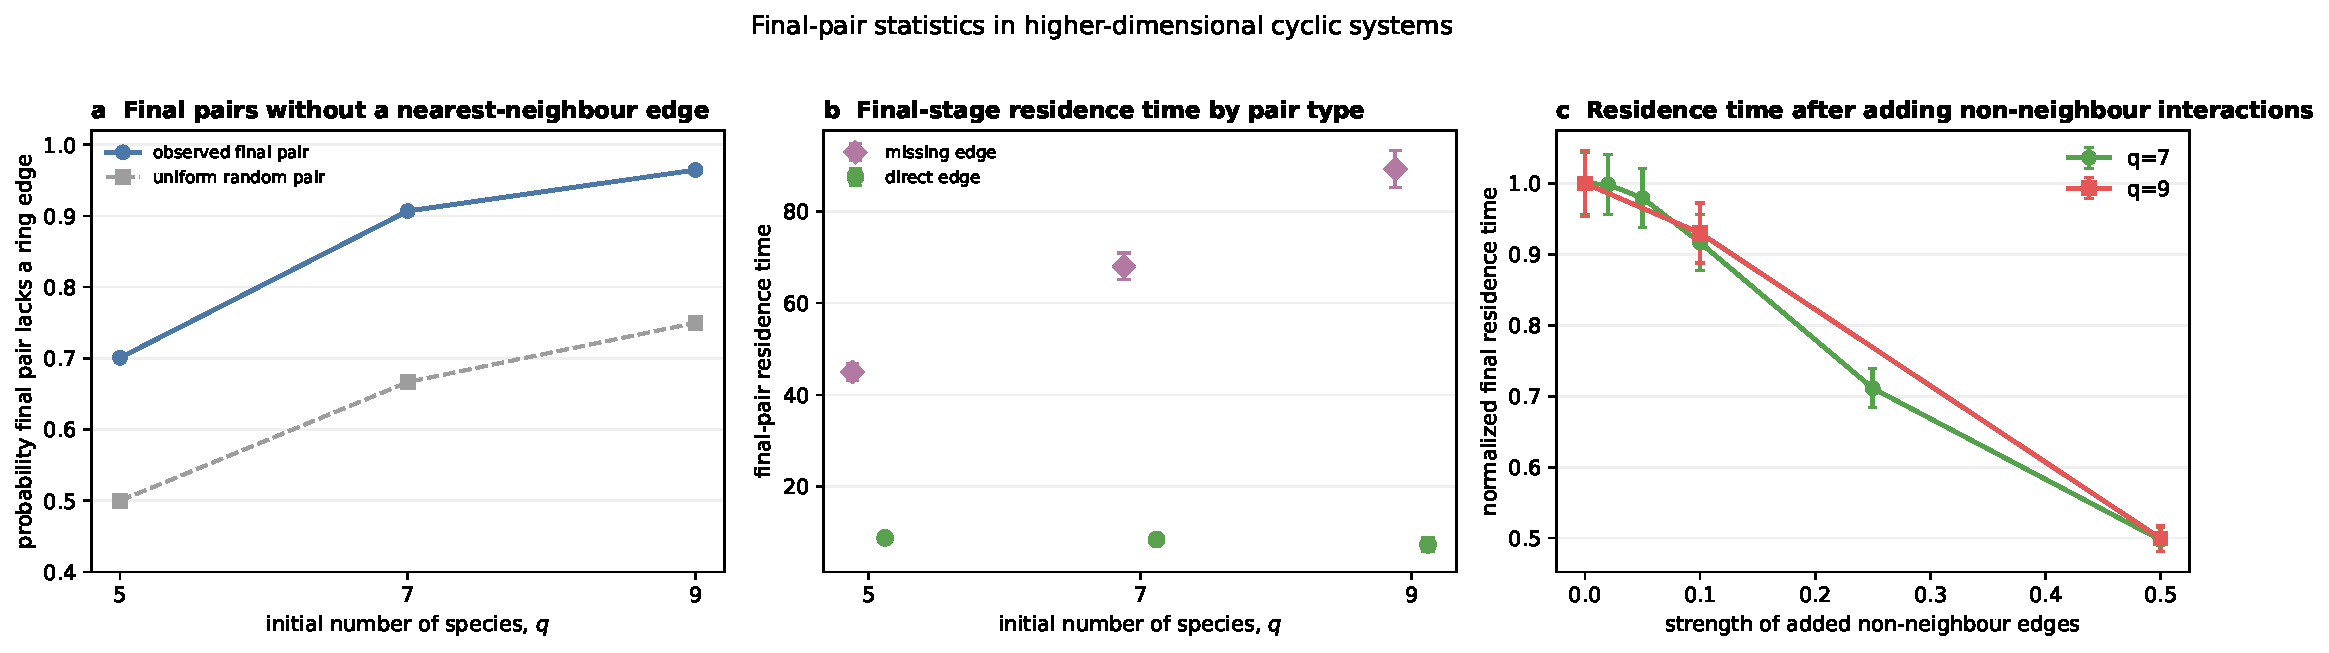
\includegraphics[width=\textwidth]{fragmentation_core_result.pdf}
  \caption{Observed final-pair statistics. Error bars in panels b and c are 95\% normal intervals ($1.96\,\se$). Panel a compares the observed fraction with the combinatorial value for a uniformly sampled pair. Panel c adds antisymmetric interactions between pairs that were unconnected in the nearest-neighbour ring; residence times are normalized by the value at zero added-edge strength.}
  \label{fig:main}
\end{figure}

\paragraph{Numerical observations.}
The final pair lacks a nearest-neighbour interaction edge in $0.7008$, $0.9068$, and $0.9645$ of the trajectories for $q=5,7,9$, respectively (Fig.~\ref{fig:main}a).  The corresponding fractions for a uniformly sampled unordered pair are $0.5000$, $0.6667$, and $0.7500$.  The counts are $2803/4000$, $2267/2500$, and $1929/2000$; one-sided binomial tail probabilities relative to those combinatorial values are below $2.2\times10^{-146}$ in each case.

Final pairs without a ring edge also remain for longer before fixation (Fig.~\ref{fig:main}b):
\begin{center}
\small
\begin{tabular}{@{}cccc@{}}
\toprule
$q$ & trajectories & no ring edge, mean $\pm\se$ & ring edge present, mean $\pm\se$\\
\midrule
5 & 4000 & $45.03\pm0.94$ & $8.80\pm0.20$\\
7 & 2500 & $68.00\pm1.49$ & $8.45\pm0.42$\\
9 & 2000 & $89.20\pm2.08$ & $7.31\pm0.80$\\
\bottomrule
\end{tabular}
\end{center}
Thus, in these runs, the ratio of the two conditional means changes from $5.11$ to $8.05$ to $12.21$ as $q$ increases.

To check how the final-stage timing changes when the absent interactions are introduced, I retained the original ring and added weighted antisymmetric edges between previously unconnected pairs.  At added-edge strength $0.5$, the unconditional mean final-pair residence time changes from $62.45$ to $31.07$ for $q=7$, and from $86.29$ to $43.11$ for $q=9$ (Fig.~\ref{fig:main}c).  The intermediate $q=7$ values at strengths $0.10$ and $0.25$ are $57.23$ and $44.42$.

\paragraph{Checks and scope.}
At $q=7$, the separation between pairs without and with a ring edge remains visible after changing the switching amplitude from $0.7$ to $0.5$ (conditional means $67.87$ and $8.09$) and after changing the switching rate from $20$ to $40$ ($66.42$ and $7.27$).  A separately written NumPy Gillespie implementation was also compared with the optimized Node implementation in a three-species benchmark; four Monte Carlo homogeneity tests gave $p=0.815,0.153,0.512,0.846$.

These calculations concern one family of weighted odd cycles and one way of adding the missing edges.  They do not determine whether the same final-pair pattern occurs for other sparse interaction graphs, other initial conditions, or other environmental processes.  The code, seeds, processed outputs, and plotting script accompanying this note are included so that the displayed comparisons can be inspected and rerun.

\vspace{2pt}
\begin{thebibliography}{9}\small
\bibitem{west2018} R. West, M. Mobilia and A. M. Rucklidge, ``Survival behavior in the cyclic Lotka--Volterra model with a randomly switching reaction rate,'' \emph{Phys. Rev. E} \textbf{97}, 022406 (2018).
\bibitem{west2020} R. West and M. Mobilia, ``Fixation properties of rock-paper-scissors games in fluctuating populations,'' \emph{J. Theor. Biol.} \textbf{491}, 110135 (2020).
\end{thebibliography}

\end{document}
